\section{Disk Arrangements}\label{sec:disk}

 A \textit{disk arrangement} is a set of interior disjoint disks, $D$.  
 If for any pair of disks in $D$ intersect at a boundary point, they are said to be in contact (kissing).

\begin{minipage}{\linewidth}
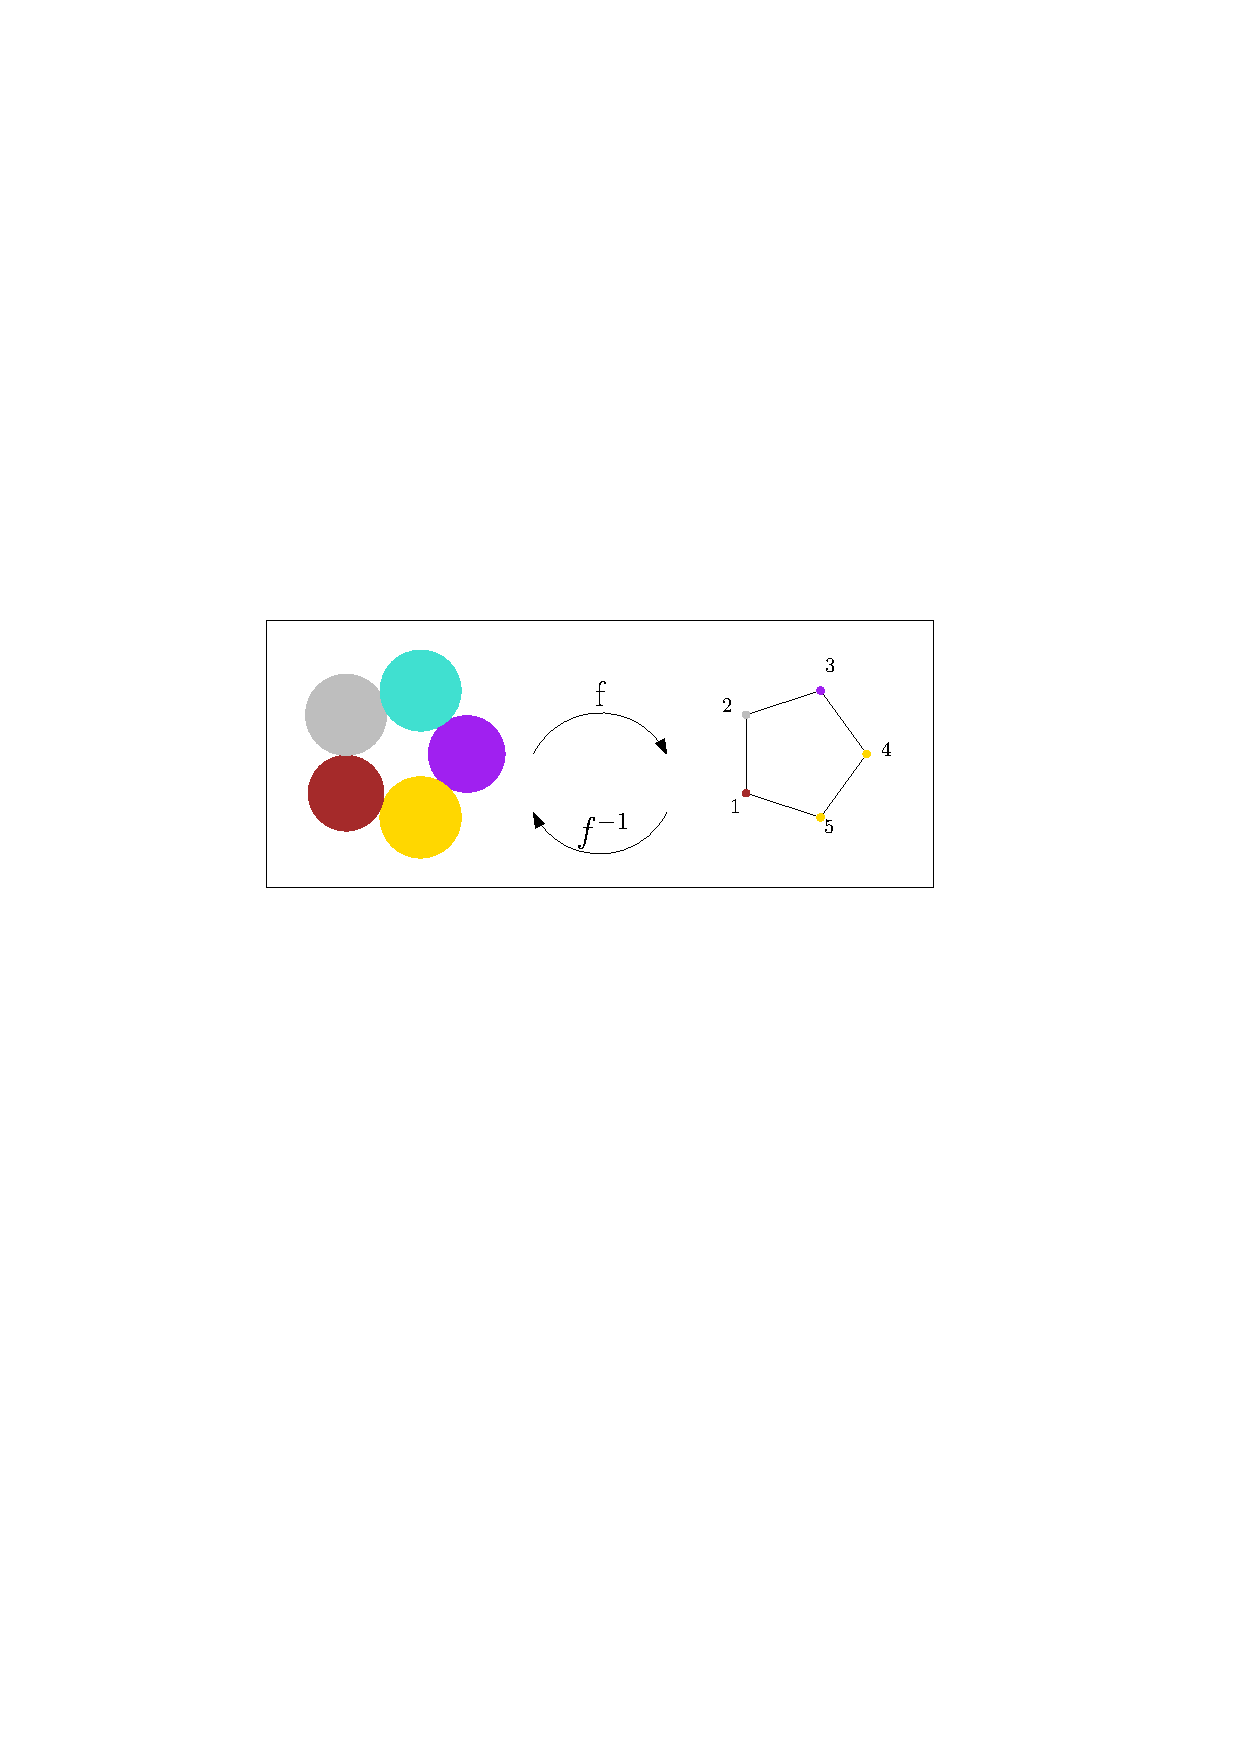
\includegraphics[scale=1]{graphics/diskPackingTheoremExample.pdf}
\captionof{figure}{This example represents a disk arrangement and its contact graph.}
\label{fig:DiskArrangement-1}
\end{minipage}

A \textit{contact graph} $G=(V,E)$ corresponding to a given disk arrangement where there is a bijection $b_V: V \mapsto D$ and a bijection that maps an edge $e_{i,j} \in E$ to an interior disjoint pair of disks $d_i$, $d_j \in D$ (see Figure \ref{fig:DiskArrangement-1}).
Given a disk arrangement, the contact graph can be thought of as a linkage because the distance between two kissing disk equal the sum of radii.  
However if the two disks don't kiss, the distance between their centers is strictly greater than the sum of their radii.
Given a disk arrangement, the contact graph can be thought of as a linkage because the distance between two kissing disk equal the sum of radii.  
However if the two disks don't kiss, the distance between their centers is strictly greater than the sum of their radii.

Koebe's theorem states that for every planar graph $G$, there exists a planar disk arrangement whose contact graph is $G$ \cite{koebe1936kontaktprobleme}.
This motivates the question of whether a planar graph $G$ is a contact graph of a disk arrangement with given radii.
The radii can be given by a weight function.
Let $\omega: V \mapsto \bbR^+$ be the \textit{weight function}.  
$\omega$ assigns a weight to each vertex in $V$.  
Let $\Pi:V \mapsto \bbr^2$ be that planar mapping of vertices.

For planar graphs with positive weighted vertices, we pose two realizability problems:
\begin{prob}[Unordered Realizibility Problem for a Contact Graph]\label{problem:UnorderedContactGraph}
Given a planar graph with positive weighted vertices, is it a contact graph of some disk arrangement where the radii equal the vertex weights?
\end{prob}
\begin{prob}[Ordered Realizibility Problem for a Contact Graph]\label{problem:OrderedContactGraph}
Given a planar graph with positive weighted vertices and a combinatorial embedding, is it a contact graph of some disk arrangement where the radii equal the vertex weights and the counter-clockwise order of neighbors of each disk is specified by the combinatorial embedding?
\end{prob}

An instance of Problem \ref{problem:UnorderedContactGraph} is shown in Figure \ref{fig:DiskArrangement-1} where the cycle graph $C_5$ is the contact graph of unit disks.
It is not difficult to see that there exists a planar graph with positive weights with no realizable disk arrangement.
Consider the a star graph with 6 leafs, each vertex with unit weight.
In any realization, the angle between two consecutive edges must be greater than $\frac{\pi}{3}$. 
The sum of 6 angles is $2 \pi$ however, the sum of 6 consecutive angles is greater than $2\pi$.
The contradiction shows that no realization is possible (refer to Figure \ref{figure:starweel}).
Note that with the wheel graph $W_7$ is realizable as a contact graph of unit disks.

Every path with arbitrary positive radii is realizable as a contact graph, place the vertices on a line.
We show that not all binary trees are realizable, even with unit disks.% of unit radii.
Consider the balanced binary trees of depth $i$ $\left\lbrace T_i \right\rbrace_{i=1}^\infty$ with unit weights on the vertices (see Figure \ref{fig:circlePacking-1}).
These trees are not realizable for sufficiently large $i$.
\begin{figure}[!htbp]
\begin{center}
  \begin{subfigure}[b]{0.21\textwidth}
	  \includegraphics[width=\textwidth]{graphics/BinaryTree1.pdf}
	  \caption{Binary tree $T_2$.}
	  \label{fig:circlePacking1-1}
  \end{subfigure}
  \begin{subfigure}[b]{0.21\textwidth}
	  \includegraphics[width=\textwidth]{graphics/BinaryTree2.pdf}
	  \caption{Binary tree $T_3$.}
	  \label{fig:circlePacking1-2}
  \end{subfigure}
  \begin{subfigure}[b]{0.21\textwidth}
	  \includegraphics[width=\textwidth]{graphics/BinaryTree3.pdf}
	  \caption{Binary tree $T_4$.}
	  \label{fig:circlePacking1-3}
  \end{subfigure}
  \begin{subfigure}[b]{0.21\textwidth}
	  \includegraphics[width=\textwidth]{graphics/BinaryTree4.pdf}
	  \caption{Binary tree $T_5$.}
	  \label{fig:circlePacking1-4}
  \end{subfigure}
  \caption{ We show the linkages $T_2$ through $T_5$ with distance 2 between adjacent vertices.  }\label{fig:circlePacking-1}
\end{center} 
\end{figure}
Let $i$ be a positive integer and suppose that $T_i$ is a contact graph of unit disks.
The balanced binary tree $T_i$ has $2^i -1$ vertices.
The total area of the disks is $\left( 2^i -1 \right)^2 \cdot \pi$.
We now derive an upper bound for this area.
Suppose the disk corresponding to the root of the tree is centered at the origin.
The centers of the disks at level $j$ are at a distance at most $2\cdot (j-1)$ away from the origin.
The centers of all disks are at distance at most $2 \cdot (i -1)$ away from the origin.
All unit disks are contained in a disk of radius $2i-1$ centered at the origin.
The total area of the disks is at most $(2i-1)^2$.  
A upper bound of the total area of the disk arrangement is the area of the bounding box of the disks.

\begin{figure}[!htpb]\label{fig:circlePacking-2}
\begin{center}
  \begin{subfigure}[b]{0.24\textwidth}
	  
\includegraphics[width=\textwidth]{graphics/degree2arrangement.pdf}
	  \caption{A disk arrangement with two layers of disks}
	  \label{fig:circlePacking2-1}
  \end{subfigure}
  \begin{subfigure}[b]{0.24\textwidth}
	  
\includegraphics[width=\textwidth]{graphics/degree3arrangement.pdf}
	  \caption{A disk arrangement with three layers of disks}
	  \label{fig:circlePacking2-2}
  \end{subfigure}
  \begin{subfigure}[b]{0.24\textwidth}
	  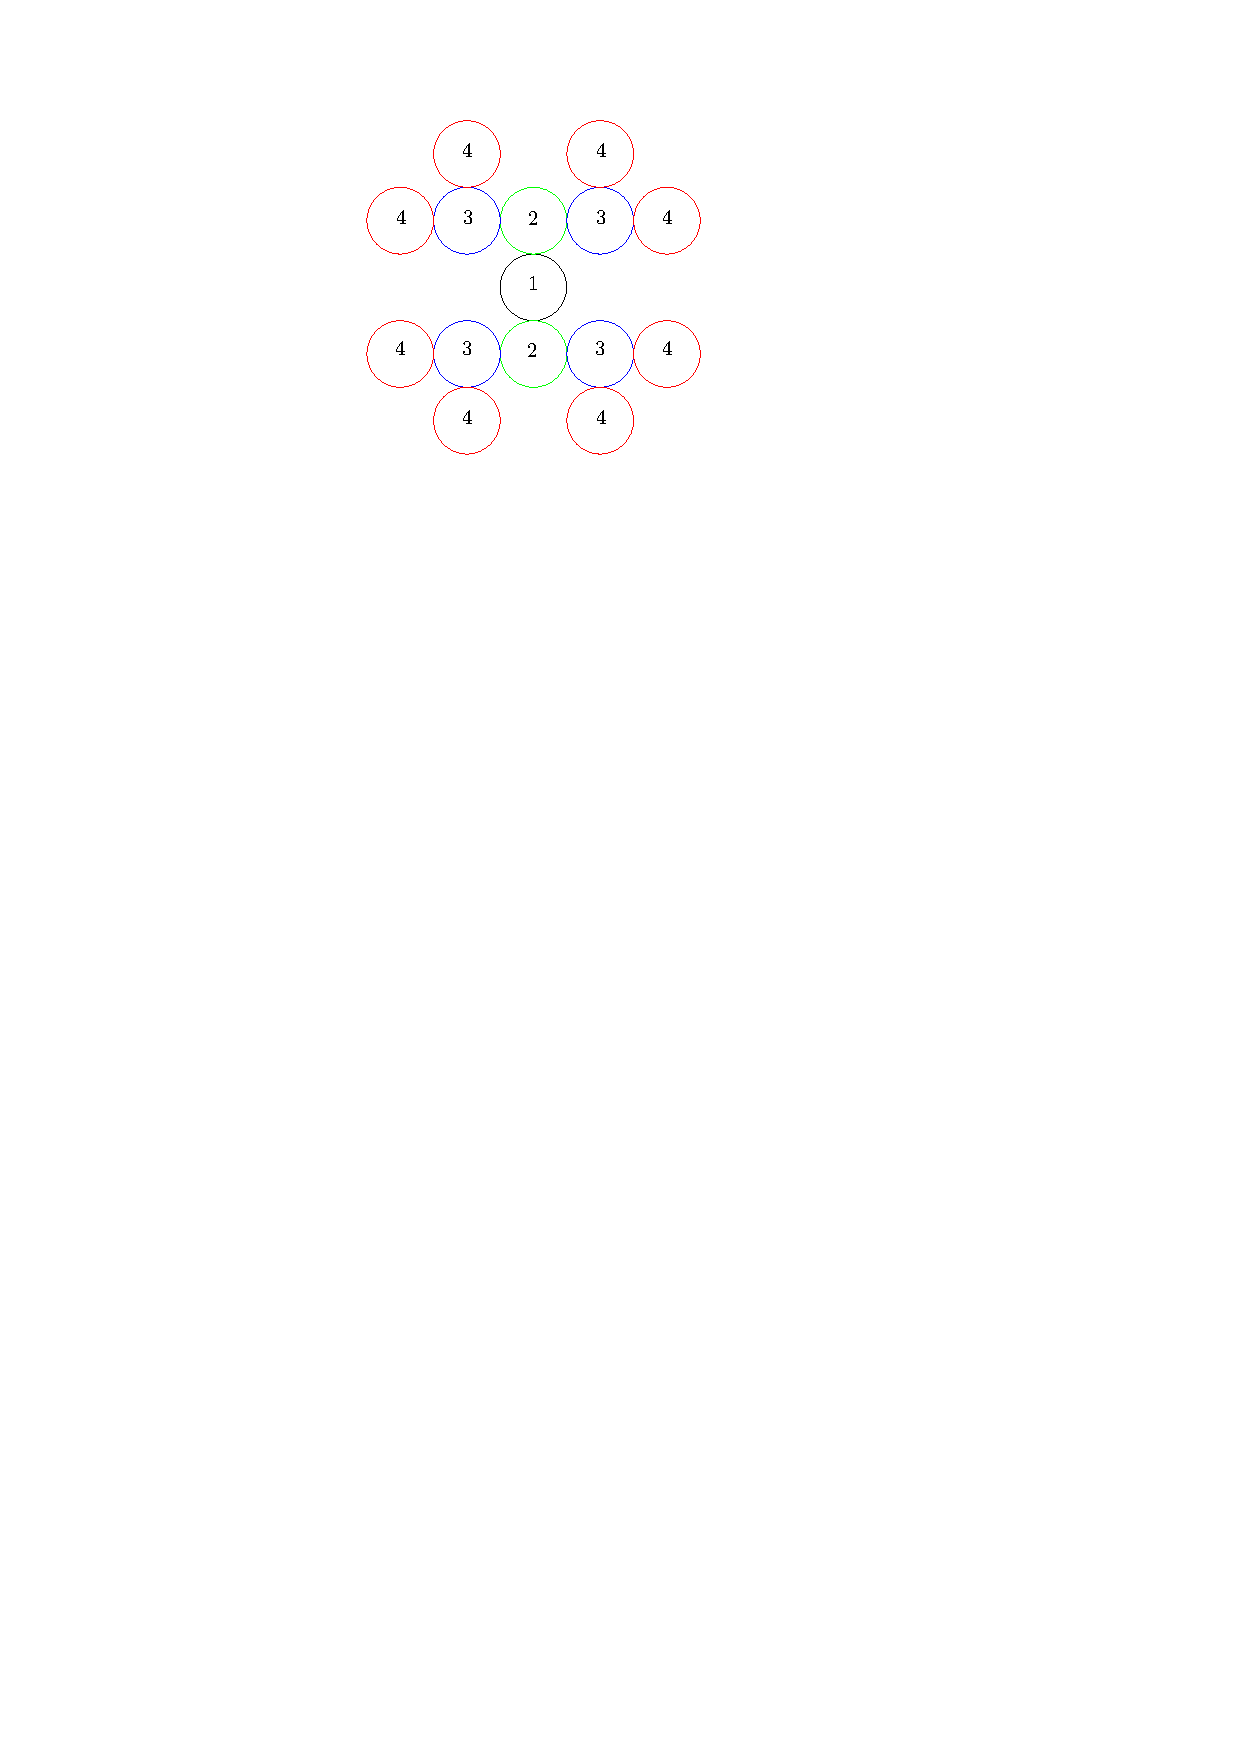
\includegraphics[width=\textwidth]{graphics/degree4arrangement.pdf}
	  \caption{A disk arrangement with four layers of disks}
	  \label{fig:circlePacking2-3}
  \end{subfigure}
  \begin{subfigure}[b]{0.24\textwidth}
	  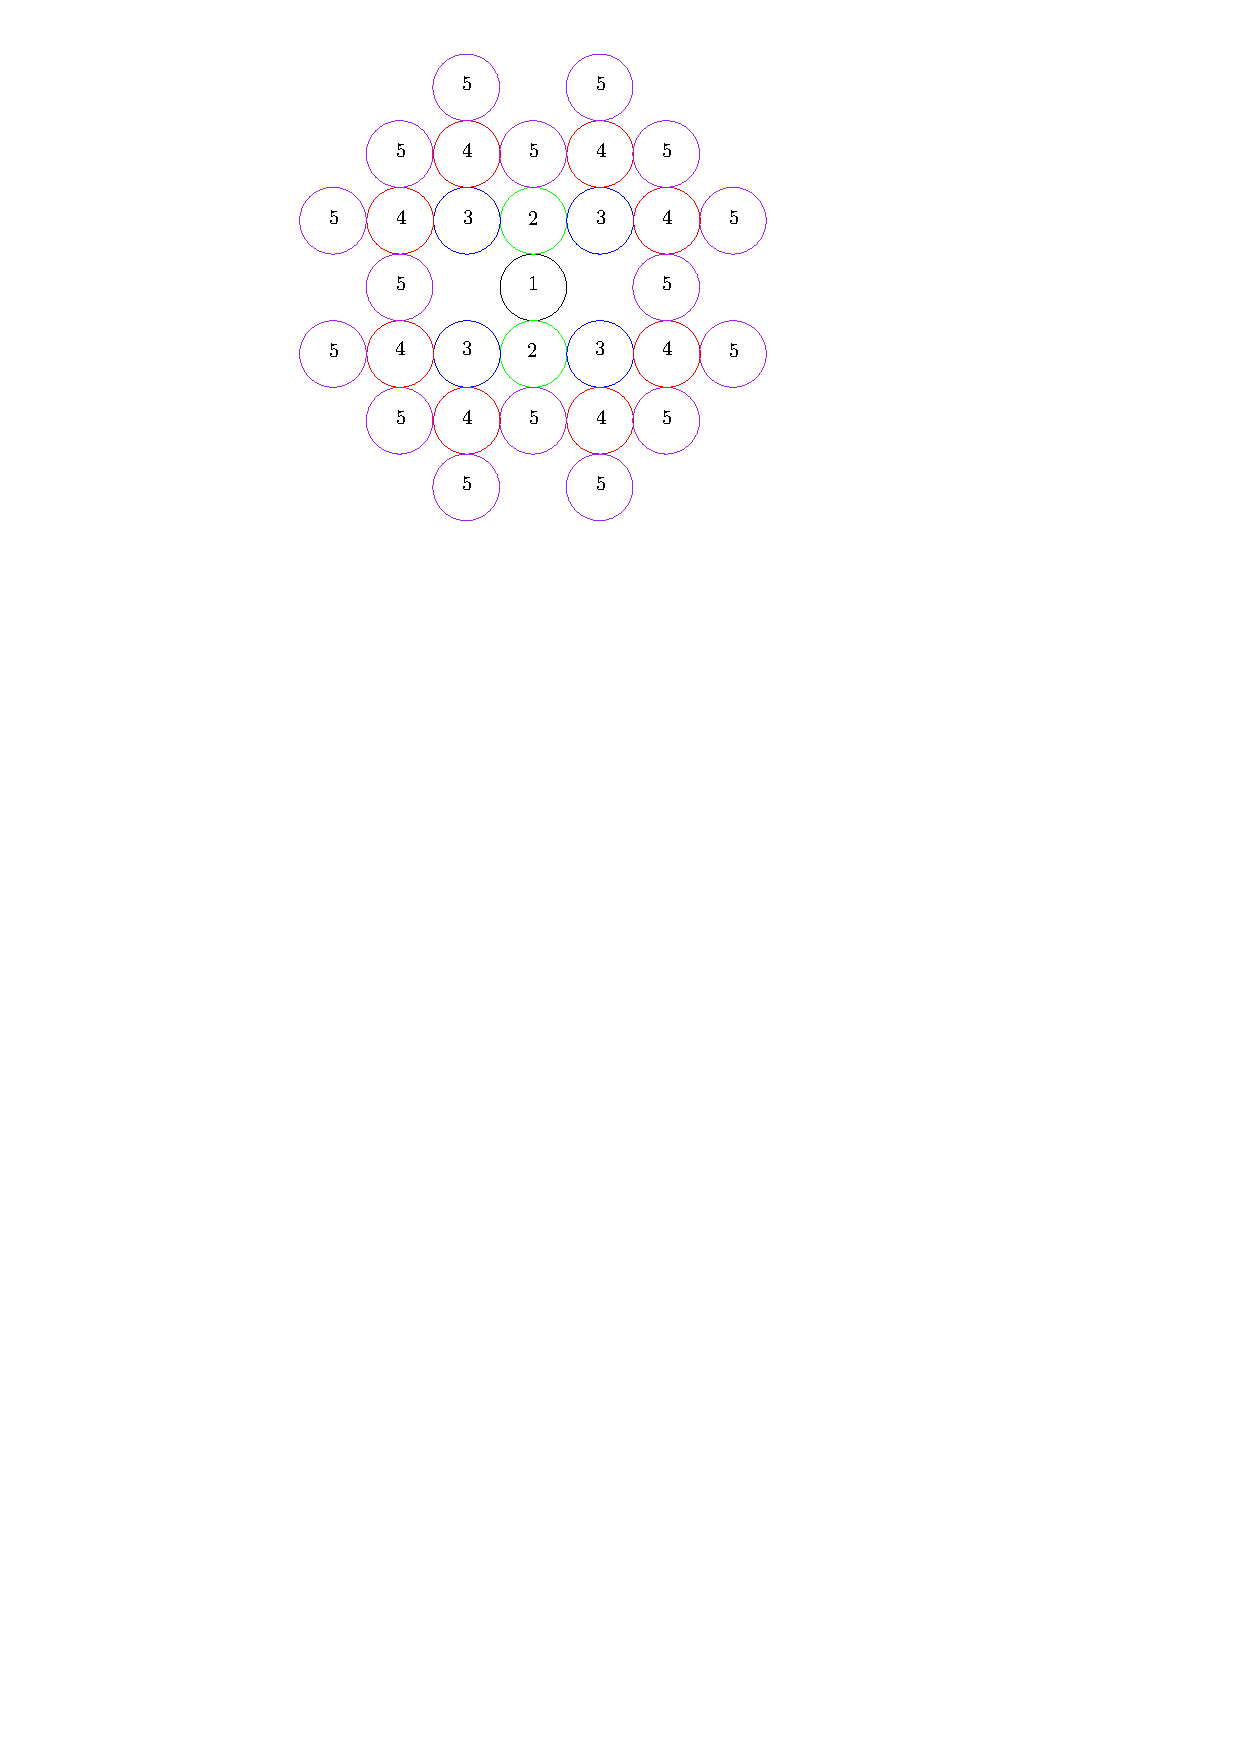
\includegraphics[width=\textwidth]{graphics/degree5arrangement.pdf}
	  \caption{A disk arrangement with five layers of disks}
	  \label{fig:circlePacking2-4}
  \end{subfigure}
\end{center} 
\caption{For $i=2,3,4,5$ the tree $T_i$ is a contact graph of unit disks.}
\end{figure}
Figure \ref{fig:circlePacking-2} shows the first four non-trivial trees as a contact graph of unit disks.
Every disk at level up to $i$ is contained in a disk of radius $2\cdot i - 1$ centered at the origin.
The total area of the disk arrangement is $(2\cdot i -1)^2 \cdot \pi$. 
When $i\geq 8$ we have a contradiciton.

\begin{figure}[!htbp]
\begin{center}
  \begin{subfigure}[b]{.48\textwidth}
  \begin{center}
	  \includegraphics[scale=.9]{graphics/OrderedDiskArrangementExample1.pdf}
	  \label{fig:circlePacking3-1}
	  \end{center}
  \end{subfigure}
  \begin{subfigure}[b]{0.48\textwidth}
  \begin{center}
	  \includegraphics[scale=.9]{graphics/OrderedDiskArrangementExample2.pdf}	  
	  \label{fig:circlePacking3-2}
	  \end{center}
  \end{subfigure}
  \caption{Consider these two ordered disk arrangements where A and B are in the concentric rings of disks.  The large disks are in contact to A and B respectively.  
  If A and B are adjacent, then there is a restriction of how large the size of the disks can be that are attached to them as seen in on the left.  
  Whereas if A and B are not adjacent in this disk arrangment as shown on the right, the size of the kissings disks could be arbitrarily large.}\label{fig:circlePacking-3}
\end{center} 
\end{figure}

There are instances where a planar graph with weights admits a realization but the cyclic order of neighbors may not be the same as the combinatorial embedding.
Define $G$ as follows: start with a star centered at $C$ and with 6 leafs, $A_1$ through $A_6$; attach two leafs, $B_1$ and $B_2$, to $A_1$ and  $A_2$ respectively (see  Figure \ref{fig:circlePacking-3}).
Let the weight of $C$ be $1+\epsilon$ for sufficiently small $\epsilon > 0$.
The neighbors of $C$ have unit weight.
The weights of the two leaves have weight $\frac{1}{\epsilon}$.  
The right of Figure \ref{fig:circlePacking-3}) shows a realization where $A_1$ and $A_2$ are in opposite position of the counter-clockwise order around $C$.
If $A_1$ and $A_2$ are required to be consecutive in the counter-clockwise order around $C$, there is no realization.

Suppose there is a realization where $A_1, \ldots, A_6$ are in the counter-clockwise order around $C$ (see Figure \ref{fig:DiskArrangement-4}).
If $\epsilon>0$ is sufficiently small, then the centers of of $A_1, \ldots, A_6$ are arbitrarily close to the vertices of a regular hexagon.
Consider the common tangent lines between $A_1$ and $B_1$ and $A_2$ and $B_2$.
The possible position of tangent line between $A_1$ and $B_1$ ranges from the common tangent line of $A_1$ and $A_6$ to the common tangent line of $A_1$ and $A_2$.
Similarly, The possible position of tangent line between $A_2$ and $B_2$ ranges from the common tangent line of $A_2$ and $A_3$ to the common tangent line of $A_1$ and $A_2$.
In any position, the common tangent lines between $A_1$ and $B_1$ and $A_2$ and $B_2$ intersect.
If $\frac{1}{\epsilon}$ is sufficiently large, then the disks $D_1$ and $D_2$ also intersect.
This contradicts that there is a realization.

\begin{minipage}{\linewidth}
\begin{center}
\includegraphics[width=.4\columnwidth]{graphics/orderedPlaneIntersection.pdf}
\end{center}
\captionof{figure}{This example represents a disk arrangement and its contact graph.}
\label{fig:DiskArrangement-4}
\end{minipage}

Figure \ref{fig:circlePacking-3} shows how an ordered contact graph may not be realizable.  
On the left, it shows a limitation on the weights of the disks that are in contact with disks A and B. 
On the right, the figure shows the order where A and B are on opposing ends of the ring of disks and can allow of arbitrary size of wieghted disks in contact with A and B.
